\section{Основы кинематики}

\df{Материальная точка}{объект, размерами которого можно пренебречь.
\[
    \vec{r}(t) = \vc{x}{y}{z} \text{;} \quad
    \vec{v} = \deriv{\vec{r}}{t} = \vc{\dot{x}}{\dot{y}}{\dot{z}} \text{;} \quad
    \vec{a} = \deriv{\vec{v}}{t} = \deriv[2]{\vec{r}}{t} = \vc{\ddot{x}}{\ddot{y}}{\ddot{z}}
\]
}

\begin{example}
Пусть точка движется по окружности радиусом $R$, угловая скорость -- $\omega$.

\[ \vec{r} = \vb{R \cos{\omega t}}{R \sin{\omega t}} \]
\[ \vec{v} = \deriv{\vec{r}}{t} = \vb{-R \omega \sin{\omega t}}{R \omega \cos{\omega t}} \]
\[ \vec{a} = \deriv{\vec{v}}{t} = \vb{-R \omega^2 \cos{\omega t}}{-R \omega^2 \sin{\omega t}} = -\vec{r} \omega^2 \]

\end{example}

Пусть $s(t)$ -- длина дуги, уже пройдённой объектом; $r(s)$ -- радиус-вектор точки, в которой он оказался.

\df{Касательный вектор}{единичный вектор, направленный по касательной к траектории.
\[ \vec{\tau} = \deriv{\vec{r}}{s} \]
}

\[ \vec{v}(t) = \deriv{\vec{r}}{t} = \deriv{\vec{r}}{s} \deriv{s}{t} = v \deriv{\vec{r}}{s} = v \vec{\tau} \]

\begin{wrapfigure}{r}{0.2\textwidth}
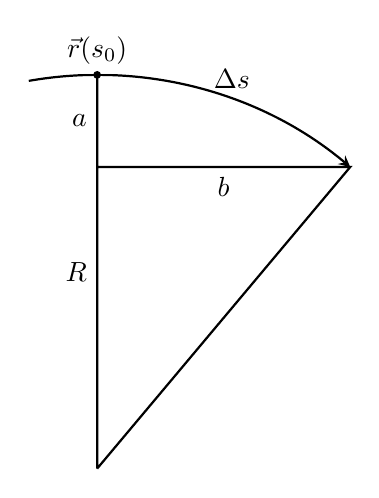
\begin{tikzpicture}[scale=5,thick]
\draw[stealth-] ({cos(50)}, {sin(50)}) arc (50:100:1);
\draw   (0,0) -- (0,1)
        (0,0) -- ({cos(50)}, {sin(50)}) -- (0, {sin(50)});

\coordinate (A) at ({cos(50)}, {sin(50)}) {};
\coordinate (B) at (0, 1) {};
\coordinate (C) at (0, {sin(50)}) {};

\tkzMarkRightAngle[size=0.035](A,C,B);
\draw (0,1) node[above,fill=white,fill opacity=0.85,text opacity=1]{{$\vec{r}(s_0)$}}
    node[circle,fill=black,inner sep=1](0,1){}
    (0,0.5) node[left]{{$R$}}
    ({cos(70)}, {sin(70)}) node[above]{{$\Delta s$}}
    (0,{1-(1-sin(50))/2}) node[left]{{$a$}}
    ({cos(50)/2},{sin(50)}) node[below]{{$b$}};
\end{tikzpicture}
\end{wrapfigure}

Аппроксимируем траекторию точки вблизи $(s_0, \; \vec{r}(s_0))$ многочленом Тейлора степени 2.

\[ \vec{r}(s) = \vec{r}(s_0) + \deriv{\vec{r}}{s}(s_0) \Delta s + \frac{\dlta^2 \vec{r}}{2 \dlta s^2}(s_0) \Delta s^2 \]

Путём медитации над картинкой можно получить ($(s_0)$ в формулах опущено)
\[
    a = \abs{\frac{\dlta^2 \vec{r}}{2 \dlta s^2} \Delta s^2}; \quad
    b = \abs{\deriv{\vec{r}}{s} \Delta s}; \quad
    R = \frac{b^2}{2a} + \frac{a}{2}
\]
\[ R = \frac{\left( \deriv{\vec{r}}{s} \Delta s \right)^2}{2 \abs{\frac{\dlta^2 \vec{r}}{2 \dlta s^2} \Delta s^2}} + \abs{\frac{\frac{\dlta^2 \vec{r}}{2 \dlta s^2} \Delta s^2}{2}} = \frac{\abs{\dlta \vec{r}\, ^2}}{\abs{\dlta^2 \vec{r} \,}} + \abs{\frac{\dlta^2 \vec{r}}{4 \dlta s^2} \Delta s^2} = \frac{\abs{\dlta \vec{r}\, ^2}}{\abs{\dlta^2 \vec{r} \,}} \]
\[ \abs{\dlta^2 \vec{r}\,} = \frac{\abs{\dlta \vec{r}\, ^2}}{R} \]

\[ \vec{a}(t) =
    \deriv{}{t}( v \vec{\tau} ) =
    \deriv{v}{t} \vec{\tau} + v \deriv{\vec{\tau}}{t} =
    a \vec{\tau} + v \deriv{\vec{\tau}}{t} =
    a \vec{\tau} + v \deriv{\vec{\tau}}{t} =
    a \vec{\tau} + v \deriv{\vec{\tau}}{s} \deriv{s}{t} =
    a \vec{\tau} + v^2 \deriv{\vec{\tau}}{t} =
    \]\[ =
    a \vec{\tau} + v^2 \deriv[2]{\vec{r}}{s} =
    a \vec{\tau} + v^2 \vec{n} \abs{\deriv[2]{\vec{r}}{s}} =
    a \vec{\tau} + \frac{v^2}{R} \vec{n} \abs{\frac{\dlta \vec{r}\, ^2}{\dlta s^2}} = 
    a \vec{\tau} + \frac{v^2}{R} \vec{n} \abs{\deriv{\vec{r}}{s}}^2 = 
    a \vec{\tau} + \frac{v^2}{R} \vec{n}
\]
